\documentclass[]{book}
\usepackage{lmodern}
\usepackage{amssymb,amsmath}
\usepackage{ifxetex,ifluatex}
\usepackage{fixltx2e} % provides \textsubscript
\ifnum 0\ifxetex 1\fi\ifluatex 1\fi=0 % if pdftex
  \usepackage[T1]{fontenc}
  \usepackage[utf8]{inputenc}
\else % if luatex or xelatex
  \ifxetex
    \usepackage{mathspec}
  \else
    \usepackage{fontspec}
  \fi
  \defaultfontfeatures{Ligatures=TeX,Scale=MatchLowercase}
\fi
% use upquote if available, for straight quotes in verbatim environments
\IfFileExists{upquote.sty}{\usepackage{upquote}}{}
% use microtype if available
\IfFileExists{microtype.sty}{%
\usepackage{microtype}
\UseMicrotypeSet[protrusion]{basicmath} % disable protrusion for tt fonts
}{}
\usepackage[margin=1in]{geometry}
\usepackage{hyperref}
\hypersetup{unicode=true,
            pdftitle={Cartographie avec R},
            pdfauthor={Timothée Giraud \& Hugues Pécout},
            pdfborder={0 0 0},
            breaklinks=true}
\urlstyle{same}  % don't use monospace font for urls
\usepackage{natbib}
\bibliographystyle{apalike}
\usepackage{color}
\usepackage{fancyvrb}
\newcommand{\VerbBar}{|}
\newcommand{\VERB}{\Verb[commandchars=\\\{\}]}
\DefineVerbatimEnvironment{Highlighting}{Verbatim}{commandchars=\\\{\}}
% Add ',fontsize=\small' for more characters per line
\usepackage{framed}
\definecolor{shadecolor}{RGB}{248,248,248}
\newenvironment{Shaded}{\begin{snugshade}}{\end{snugshade}}
\newcommand{\AlertTok}[1]{\textcolor[rgb]{0.94,0.16,0.16}{#1}}
\newcommand{\AnnotationTok}[1]{\textcolor[rgb]{0.56,0.35,0.01}{\textbf{\textit{#1}}}}
\newcommand{\AttributeTok}[1]{\textcolor[rgb]{0.77,0.63,0.00}{#1}}
\newcommand{\BaseNTok}[1]{\textcolor[rgb]{0.00,0.00,0.81}{#1}}
\newcommand{\BuiltInTok}[1]{#1}
\newcommand{\CharTok}[1]{\textcolor[rgb]{0.31,0.60,0.02}{#1}}
\newcommand{\CommentTok}[1]{\textcolor[rgb]{0.56,0.35,0.01}{\textit{#1}}}
\newcommand{\CommentVarTok}[1]{\textcolor[rgb]{0.56,0.35,0.01}{\textbf{\textit{#1}}}}
\newcommand{\ConstantTok}[1]{\textcolor[rgb]{0.00,0.00,0.00}{#1}}
\newcommand{\ControlFlowTok}[1]{\textcolor[rgb]{0.13,0.29,0.53}{\textbf{#1}}}
\newcommand{\DataTypeTok}[1]{\textcolor[rgb]{0.13,0.29,0.53}{#1}}
\newcommand{\DecValTok}[1]{\textcolor[rgb]{0.00,0.00,0.81}{#1}}
\newcommand{\DocumentationTok}[1]{\textcolor[rgb]{0.56,0.35,0.01}{\textbf{\textit{#1}}}}
\newcommand{\ErrorTok}[1]{\textcolor[rgb]{0.64,0.00,0.00}{\textbf{#1}}}
\newcommand{\ExtensionTok}[1]{#1}
\newcommand{\FloatTok}[1]{\textcolor[rgb]{0.00,0.00,0.81}{#1}}
\newcommand{\FunctionTok}[1]{\textcolor[rgb]{0.00,0.00,0.00}{#1}}
\newcommand{\ImportTok}[1]{#1}
\newcommand{\InformationTok}[1]{\textcolor[rgb]{0.56,0.35,0.01}{\textbf{\textit{#1}}}}
\newcommand{\KeywordTok}[1]{\textcolor[rgb]{0.13,0.29,0.53}{\textbf{#1}}}
\newcommand{\NormalTok}[1]{#1}
\newcommand{\OperatorTok}[1]{\textcolor[rgb]{0.81,0.36,0.00}{\textbf{#1}}}
\newcommand{\OtherTok}[1]{\textcolor[rgb]{0.56,0.35,0.01}{#1}}
\newcommand{\PreprocessorTok}[1]{\textcolor[rgb]{0.56,0.35,0.01}{\textit{#1}}}
\newcommand{\RegionMarkerTok}[1]{#1}
\newcommand{\SpecialCharTok}[1]{\textcolor[rgb]{0.00,0.00,0.00}{#1}}
\newcommand{\SpecialStringTok}[1]{\textcolor[rgb]{0.31,0.60,0.02}{#1}}
\newcommand{\StringTok}[1]{\textcolor[rgb]{0.31,0.60,0.02}{#1}}
\newcommand{\VariableTok}[1]{\textcolor[rgb]{0.00,0.00,0.00}{#1}}
\newcommand{\VerbatimStringTok}[1]{\textcolor[rgb]{0.31,0.60,0.02}{#1}}
\newcommand{\WarningTok}[1]{\textcolor[rgb]{0.56,0.35,0.01}{\textbf{\textit{#1}}}}
\usepackage{longtable,booktabs}
\usepackage{graphicx,grffile}
\makeatletter
\def\maxwidth{\ifdim\Gin@nat@width>\linewidth\linewidth\else\Gin@nat@width\fi}
\def\maxheight{\ifdim\Gin@nat@height>\textheight\textheight\else\Gin@nat@height\fi}
\makeatother
% Scale images if necessary, so that they will not overflow the page
% margins by default, and it is still possible to overwrite the defaults
% using explicit options in \includegraphics[width, height, ...]{}
\setkeys{Gin}{width=\maxwidth,height=\maxheight,keepaspectratio}
\IfFileExists{parskip.sty}{%
\usepackage{parskip}
}{% else
\setlength{\parindent}{0pt}
\setlength{\parskip}{6pt plus 2pt minus 1pt}
}
\setlength{\emergencystretch}{3em}  % prevent overfull lines
\providecommand{\tightlist}{%
  \setlength{\itemsep}{0pt}\setlength{\parskip}{0pt}}
\setcounter{secnumdepth}{5}
% Redefines (sub)paragraphs to behave more like sections
\ifx\paragraph\undefined\else
\let\oldparagraph\paragraph
\renewcommand{\paragraph}[1]{\oldparagraph{#1}\mbox{}}
\fi
\ifx\subparagraph\undefined\else
\let\oldsubparagraph\subparagraph
\renewcommand{\subparagraph}[1]{\oldsubparagraph{#1}\mbox{}}
\fi

%%% Use protect on footnotes to avoid problems with footnotes in titles
\let\rmarkdownfootnote\footnote%
\def\footnote{\protect\rmarkdownfootnote}

%%% Change title format to be more compact
\usepackage{titling}

% Create subtitle command for use in maketitle
\newcommand{\subtitle}[1]{
  \posttitle{
    \begin{center}\large#1\end{center}
    }
}

\setlength{\droptitle}{-2em}

  \title{Cartographie avec R}
    \pretitle{\vspace{\droptitle}\centering\huge}
  \posttitle{\par}
    \author{Timothée Giraud \& Hugues Pécout}
    \preauthor{\centering\large\emph}
  \postauthor{\par}
      \predate{\centering\large\emph}
  \postdate{\par}
    \date{2018-12-12}

\usepackage{booktabs}

\begin{document}
\maketitle

{
\setcounter{tocdepth}{1}
\tableofcontents
}
\hypertarget{introduction}{%
\chapter*{Introduction}\label{introduction}}
\addcontentsline{toc}{chapter}{Introduction}

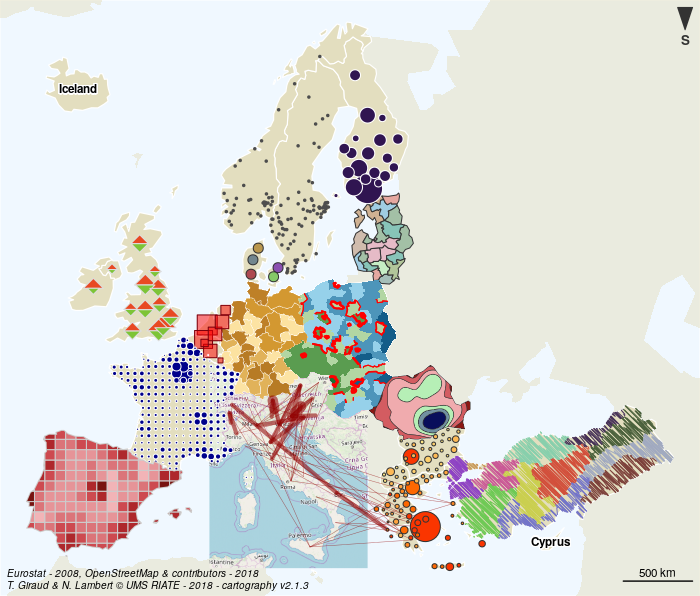
\includegraphics{img/cartomix.png}

Voici le document associé au cours de cartographie avec R.

Pour suivre ce cours vous aurez besoin des dernières versions de R et de RStudio.\\
Vous aurez aussi besoin d'un certain nombre de \emph{packages} additionels :

\begin{itemize}
\tightlist
\item
  sf
\item
  cartography
\item
  osrm
\item
  mapview
\item
  SpatialPosition
\item
  mapinsetr
\item
  raster
\item
  linemap
\item
  spatstats
\item
  \ldots{}
\end{itemize}

Ce cours ce déroule sur 3 jours :

\begin{itemize}
\tightlist
\item
  Jour 1 - \protect\hyperlink{jour1}{Les données spatiales}\\
\item
  Jour 2 - \protect\hyperlink{jour2}{Cartographie thématique}\\
\item
  Jour 3 - \protect\hyperlink{jour3}{Cartographie thématique avancée}
\end{itemize}

\hypertarget{jour1}{%
\chapter{Les données spatiales}\label{jour1}}

Il est possible d'importer, de manipuler, de traiter, d'afficher et d'exporter des données spatiales avec R. La grande majorité des opérations de géotraitement sont disponible dans R grace au package \texttt{sf}. Il devient alors possible d'utiliser R comme un SIG.

\hypertarget{le-package-sf}{%
\section{\texorpdfstring{Le package \texttt{sf}}{Le package sf}}\label{le-package-sf}}

Trois packages ``historiques''
* \texttt{rgdal} : interface entre R et les librairies GDAL (\href{http://www.gdal.org/}{Geospatial Data Abstraction Library}) et \href{https://github.com/OSGeo/proj.4}{PROJ4}.
* \texttt{sp} : classes et methodes pour les données spatiales dans R.
* \texttt{rgeos} : accès à la librairie d'opérations spatiales GEOS (\href{http://trac.osgeo.org/geos/}{Geometry Engine - Open Source}) : area, perimeter, distances, dissolve, buffer, overlap, union, contains\ldots{}

\begin{itemize}
\item
  Les fonctionnalités de \texttt{sp}, \texttt{rgeos} et \texttt{rgdal} dans un package unique.
\item
  Manipulation plus aisée, objets plus simples
\item
  Auteur principal et \emph{maintainer} : Edzer Pebesma (auteur de \texttt{sp})
\item
  Compatible avec les syntaxes \emph{pipe} et les opérateurs du \texttt{tidyverse}.
\end{itemize}

Format des objets spatiaux \texttt{sf}

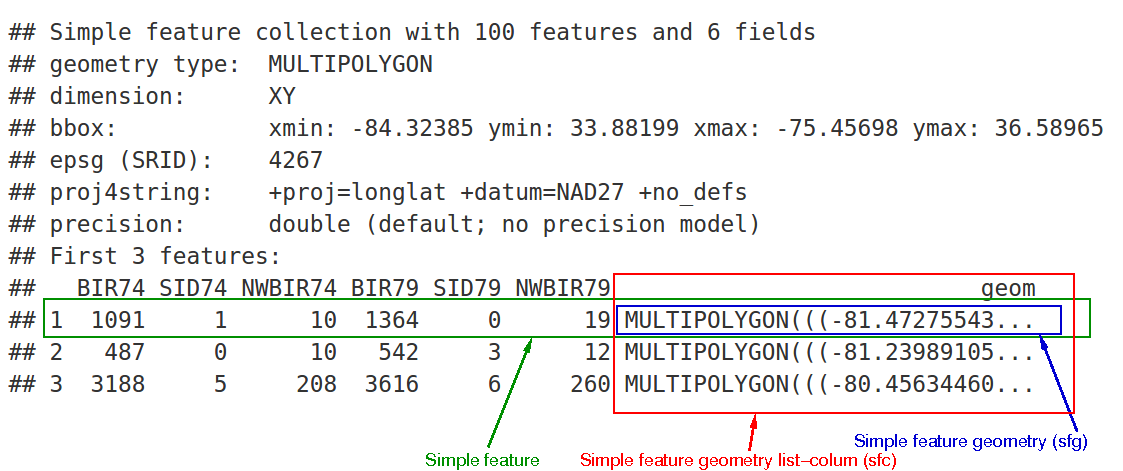
\includegraphics{img/sf.png}

Import de données

\begin{Shaded}
\begin{Highlighting}[]
\KeywordTok{library}\NormalTok{(sf)}
\NormalTok{mtq <-}\StringTok{ }\KeywordTok{st_read}\NormalTok{(}\StringTok{"data/martinique.shp"}\NormalTok{)}
\end{Highlighting}
\end{Shaded}

\begin{verbatim}
Reading layer `martinique' from data source `/home/tim/Documents/prz/carto_avec_r/data/martinique.shp' using driver `ESRI Shapefile'
Simple feature collection with 34 features and 23 fields
geometry type:  POLYGON
dimension:      XY
bbox:           xmin: 690574.4 ymin: 1592426 xmax: 736126.5 ymax: 1645660
epsg (SRID):    32620
proj4string:    +proj=utm +zone=20 +datum=WGS84 +units=m +no_defs
\end{verbatim}

Affichage de données

\begin{Shaded}
\begin{Highlighting}[]
\KeywordTok{plot}\NormalTok{(}\KeywordTok{st_geometry}\NormalTok{(mtq))}
\end{Highlighting}
\end{Shaded}

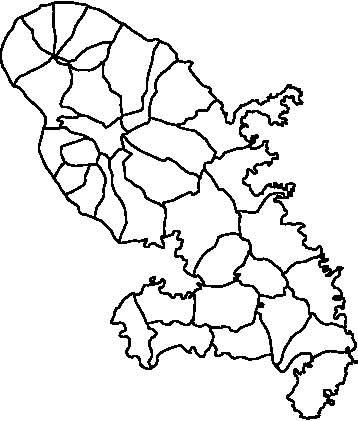
\includegraphics{Cartographie_avec_R_files/figure-latex/unnamed-chunk-2-1.pdf}

\hypertarget{import-export}{%
\section{Import / Export}\label{import-export}}

Import de données

\begin{Shaded}
\begin{Highlighting}[]
\KeywordTok{library}\NormalTok{(sf)}
\NormalTok{mtq <-}\StringTok{ }\KeywordTok{st_read}\NormalTok{(}\StringTok{"data/martinique.shp"}\NormalTok{)}
\end{Highlighting}
\end{Shaded}

\begin{verbatim}
Reading layer `martinique' from data source `/home/tim/Documents/prz/carto_avec_r/data/martinique.shp' using driver `ESRI Shapefile'
Simple feature collection with 34 features and 23 fields
geometry type:  POLYGON
dimension:      XY
bbox:           xmin: 690574.4 ymin: 1592426 xmax: 736126.5 ymax: 1645660
epsg (SRID):    32620
proj4string:    +proj=utm +zone=20 +datum=WGS84 +units=m +no_defs
\end{verbatim}

\hypertarget{les-projections}{%
\section{Les projections}\label{les-projections}}

\hypertarget{les-operations-de-geotraitement}{%
\section{Les opérations de géotraitement}\label{les-operations-de-geotraitement}}

Utiliser R comme un SIG

\begin{Shaded}
\begin{Highlighting}[]
\NormalTok{mtq_c <-}\StringTok{ }\KeywordTok{st_centroid}\NormalTok{(mtq)}
\KeywordTok{plot}\NormalTok{(}\KeywordTok{st_geometry}\NormalTok{(mtq))}
\KeywordTok{plot}\NormalTok{(}\KeywordTok{st_geometry}\NormalTok{(mtq_c), }\DataTypeTok{add=}\OtherTok{TRUE}\NormalTok{, }\DataTypeTok{cex=}\FloatTok{1.2}\NormalTok{, }\DataTypeTok{col=}\StringTok{"red"}\NormalTok{, }\DataTypeTok{pch=}\DecValTok{20}\NormalTok{)}
\end{Highlighting}
\end{Shaded}

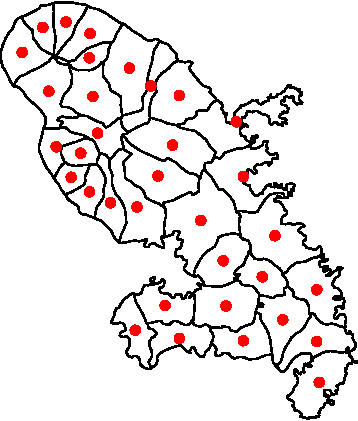
\includegraphics{Cartographie_avec_R_files/figure-latex/centroid-1.pdf}

\begin{Shaded}
\begin{Highlighting}[]
\NormalTok{mat <-}\StringTok{ }\KeywordTok{st_distance}\NormalTok{(}\DataTypeTok{x=}\NormalTok{mtq_c,}\DataTypeTok{y=}\NormalTok{mtq_c)}
\NormalTok{mat[}\DecValTok{1}\OperatorTok{:}\DecValTok{5}\NormalTok{,}\DecValTok{1}\OperatorTok{:}\DecValTok{5}\NormalTok{]}
\end{Highlighting}
\end{Shaded}

\begin{verbatim}
Units: [m]
          [,1]     [,2]      [,3]      [,4]      [,5]
[1,]     0.000 35297.56  3091.501 12131.617 17136.310
[2,] 35297.557     0.00 38332.602 25518.913 18605.249
[3,]  3091.501 38332.60     0.000 15094.702 20226.198
[4,] 12131.617 25518.91 15094.702     0.000  7177.011
[5,] 17136.310 18605.25 20226.198  7177.011     0.000
\end{verbatim}

Agréger des polygones

\begin{Shaded}
\begin{Highlighting}[]
\NormalTok{mtq_u <-}\StringTok{ }\KeywordTok{st_union}\NormalTok{(mtq)}
\KeywordTok{plot}\NormalTok{(}\KeywordTok{st_geometry}\NormalTok{(mtq), }\DataTypeTok{col=}\StringTok{"lightblue"}\NormalTok{)}
\KeywordTok{plot}\NormalTok{(}\KeywordTok{st_geometry}\NormalTok{(mtq_u), }\DataTypeTok{add=}\NormalTok{T, }\DataTypeTok{lwd=}\DecValTok{2}\NormalTok{, }\DataTypeTok{border =} \StringTok{"red"}\NormalTok{)}
\end{Highlighting}
\end{Shaded}

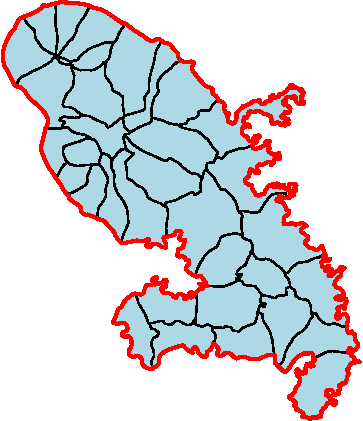
\includegraphics{Cartographie_avec_R_files/figure-latex/aggreg-1.pdf}

Construire une zone tampon

\begin{Shaded}
\begin{Highlighting}[]
\NormalTok{mtq_b <-}\StringTok{ }\KeywordTok{st_buffer}\NormalTok{(}\DataTypeTok{x =}\NormalTok{ mtq_u, }\DataTypeTok{dist =} \DecValTok{5000}\NormalTok{)}
\KeywordTok{plot}\NormalTok{(}\KeywordTok{st_geometry}\NormalTok{(mtq), }\DataTypeTok{col=}\StringTok{"lightblue"}\NormalTok{)}
\KeywordTok{plot}\NormalTok{(}\KeywordTok{st_geometry}\NormalTok{(mtq_u), }\DataTypeTok{add=}\NormalTok{T, }\DataTypeTok{lwd=}\DecValTok{2}\NormalTok{)}
\KeywordTok{plot}\NormalTok{(}\KeywordTok{st_geometry}\NormalTok{(mtq_b), }\DataTypeTok{add=}\NormalTok{T, }\DataTypeTok{lwd=}\DecValTok{2}\NormalTok{, }\DataTypeTok{border =} \StringTok{"red"}\NormalTok{)}
\end{Highlighting}
\end{Shaded}

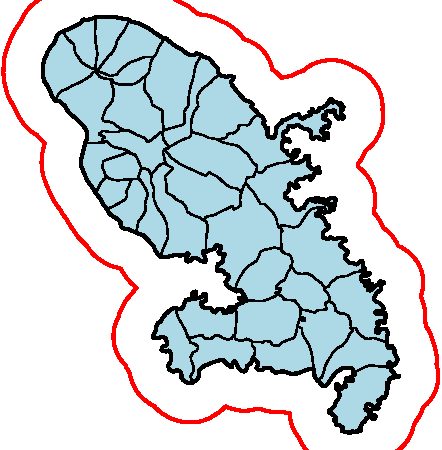
\includegraphics{Cartographie_avec_R_files/figure-latex/buffers-1.pdf}

Réaliser une intersection

\begin{Shaded}
\begin{Highlighting}[]
\NormalTok{m <-}\StringTok{ }\KeywordTok{rbind}\NormalTok{(}\KeywordTok{c}\NormalTok{(}\DecValTok{700015}\NormalTok{,}\DecValTok{1624212}\NormalTok{), }\KeywordTok{c}\NormalTok{(}\DecValTok{700015}\NormalTok{,}\DecValTok{1641586}\NormalTok{), }\KeywordTok{c}\NormalTok{(}\DecValTok{719127}\NormalTok{,}\DecValTok{1641586}\NormalTok{), }\KeywordTok{c}\NormalTok{(}\DecValTok{719127}\NormalTok{,}\DecValTok{1624212}\NormalTok{), }\KeywordTok{c}\NormalTok{(}\DecValTok{700015}\NormalTok{,}\DecValTok{1624212}\NormalTok{))}
\NormalTok{p <-}\StringTok{ }\KeywordTok{st_sf}\NormalTok{(}\KeywordTok{st_sfc}\NormalTok{(}\KeywordTok{st_polygon}\NormalTok{(}\KeywordTok{list}\NormalTok{(m))), }\DataTypeTok{crs =} \KeywordTok{st_crs}\NormalTok{(mtq))}
\KeywordTok{plot}\NormalTok{(}\KeywordTok{st_geometry}\NormalTok{(mtq))}
\KeywordTok{plot}\NormalTok{(p, }\DataTypeTok{border=}\StringTok{"red"}\NormalTok{, }\DataTypeTok{lwd=}\DecValTok{2}\NormalTok{, }\DataTypeTok{add=}\NormalTok{T)}
\end{Highlighting}
\end{Shaded}

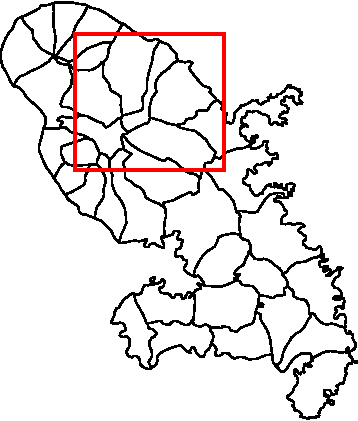
\includegraphics{Cartographie_avec_R_files/figure-latex/intersect1-1.pdf}

Réaliser une intersection

\begin{Shaded}
\begin{Highlighting}[]
\NormalTok{mtq_z <-}\StringTok{ }\KeywordTok{st_intersection}\NormalTok{(}\DataTypeTok{x =}\NormalTok{ mtq, }\DataTypeTok{y =}\NormalTok{ p)}
\KeywordTok{plot}\NormalTok{(}\KeywordTok{st_geometry}\NormalTok{(mtq))}
\KeywordTok{plot}\NormalTok{(}\KeywordTok{st_geometry}\NormalTok{(mtq_z), }\DataTypeTok{col=}\StringTok{"red"}\NormalTok{, }\DataTypeTok{border=}\StringTok{"green"}\NormalTok{, }\DataTypeTok{add=}\NormalTok{T)}
\end{Highlighting}
\end{Shaded}

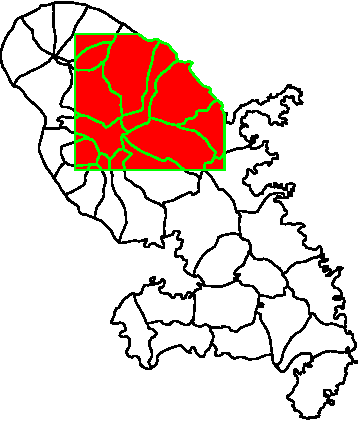
\includegraphics{Cartographie_avec_R_files/figure-latex/instersect2-1.pdf}

Construire des polygones de Voronoi
google: ``st\_voronoi R sf'' (\url{https://github.com/r-spatial/sf/issues/474} \& \url{https://stackoverflow.com/questions/45719790/create-voronoi-polygon-with-simple-feature-in-r})

\begin{Shaded}
\begin{Highlighting}[]
\NormalTok{mtq_v <-}\StringTok{ }\KeywordTok{st_voronoi}\NormalTok{(}\DataTypeTok{x =} \KeywordTok{st_union}\NormalTok{(mtq_c))}
\NormalTok{mtq_v <-}\StringTok{ }\KeywordTok{st_intersection}\NormalTok{(}\KeywordTok{st_cast}\NormalTok{(mtq_v), }\KeywordTok{st_union}\NormalTok{(mtq))}
\NormalTok{mtq_v <-}\StringTok{ }\KeywordTok{st_join}\NormalTok{(}\DataTypeTok{x =} \KeywordTok{st_sf}\NormalTok{(mtq_v), }\DataTypeTok{y =}\NormalTok{ mtq_c, }\DataTypeTok{join=}\NormalTok{st_intersects)}
\NormalTok{mtq_v <-}\StringTok{ }\KeywordTok{st_cast}\NormalTok{(mtq_v, }\StringTok{"MULTIPOLYGON"}\NormalTok{)}
\KeywordTok{plot}\NormalTok{(}\KeywordTok{st_geometry}\NormalTok{(mtq_v), }\DataTypeTok{col=}\StringTok{'lightblue'}\NormalTok{)}
\end{Highlighting}
\end{Shaded}

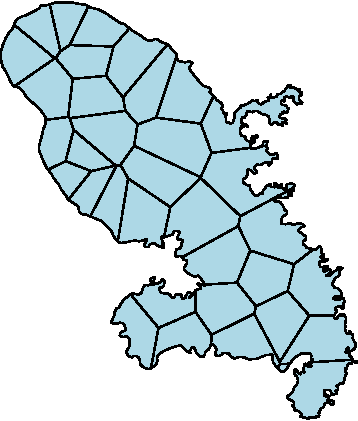
\includegraphics{Cartographie_avec_R_files/figure-latex/voronoi-1.pdf}

\hypertarget{le-package-raster}{%
\section{\texorpdfstring{Le package \texttt{raster}}{Le package raster}}\label{le-package-raster}}

\hypertarget{jour2}{%
\chapter{Cartographie thématique}\label{jour2}}

\hypertarget{le-package-cartography}{%
\section{\texorpdfstring{Le package \texttt{cartography}}{Le package cartography}}\label{le-package-cartography}}

\hypertarget{symboles-proportionnels}{%
\subsection{Symboles proportionnels}\label{symboles-proportionnels}}

\begin{Shaded}
\begin{Highlighting}[]
\KeywordTok{library}\NormalTok{(cartography)}
\KeywordTok{library}\NormalTok{(sf)}
\CommentTok{# Import des données}
\NormalTok{mtq <-}\StringTok{ }\KeywordTok{st_read}\NormalTok{(}\KeywordTok{system.file}\NormalTok{(}\StringTok{"shape/martinique.shp"}\NormalTok{, }\DataTypeTok{package=}\StringTok{"cartography"}\NormalTok{))}
\CommentTok{# Communes}
\KeywordTok{plot}\NormalTok{(}\KeywordTok{st_geometry}\NormalTok{(mtq), }\DataTypeTok{col =} \StringTok{"lightblue4"}\NormalTok{, }\DataTypeTok{border =} \StringTok{"lightblue3"}\NormalTok{, }
     \DataTypeTok{bg =} \StringTok{"lightblue1"}\NormalTok{)}
\CommentTok{# Symboles proportionnels}
\KeywordTok{propSymbolsLayer}\NormalTok{(}\DataTypeTok{x =}\NormalTok{ mtq, }\DataTypeTok{var =} \StringTok{"P13_POP"}\NormalTok{, }
                 \DataTypeTok{legend.title.txt =} \StringTok{"Total}\CharTok{\textbackslash{}n}\StringTok{population (2013)"}\NormalTok{)}
\CommentTok{# Titre}
\KeywordTok{title}\NormalTok{(}\DataTypeTok{main =} \StringTok{"Population en Martinique"}\NormalTok{)}
\end{Highlighting}
\end{Shaded}

\begin{center}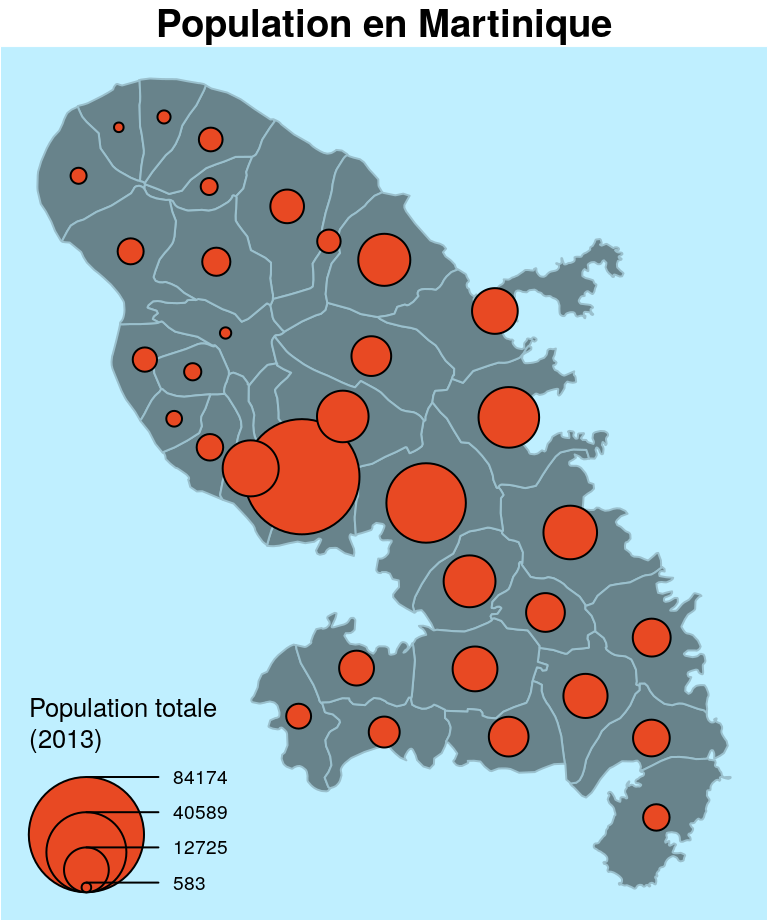
\includegraphics{Cartographie_avec_R_files/figure-latex/propS-1} \end{center}

\hypertarget{carte-choroplethe}{%
\subsection{Carte choroplèthe}\label{carte-choroplethe}}

\begin{Shaded}
\begin{Highlighting}[]
\NormalTok{mtq}\OperatorTok{$}\NormalTok{cagr <-}\StringTok{ }\NormalTok{(((mtq}\OperatorTok{$}\NormalTok{P13_POP }\OperatorTok{/}\StringTok{ }\NormalTok{mtq}\OperatorTok{$}\NormalTok{P08_POP)}\OperatorTok{^}\NormalTok{(}\DecValTok{1}\OperatorTok{/}\DecValTok{4}\NormalTok{)) }\OperatorTok{-}\StringTok{ }\DecValTok{1}\NormalTok{) }\OperatorTok{*}\StringTok{ }\DecValTok{100}
\KeywordTok{choroLayer}\NormalTok{(}\DataTypeTok{x =}\NormalTok{ mtq, }\DataTypeTok{var =} \StringTok{"cagr"}\NormalTok{, }\DataTypeTok{breaks =} \KeywordTok{c}\NormalTok{(}\OperatorTok{-}\FloatTok{6.14}\NormalTok{,}\OperatorTok{-}\DecValTok{2}\NormalTok{,}\OperatorTok{-}\DecValTok{1}\NormalTok{,}\DecValTok{0}\NormalTok{,}\DecValTok{1}\NormalTok{,}\DecValTok{2}\NormalTok{),}
           \DataTypeTok{col =} \KeywordTok{c}\NormalTok{(}\StringTok{"#135D89"}\NormalTok{, }\StringTok{"#4D95BA"}\NormalTok{, }\StringTok{"#96D1EA"}\NormalTok{, }\StringTok{"#FCDACA"}\NormalTok{, }\StringTok{"#EC4E49"}\NormalTok{),}
           \DataTypeTok{legend.title.txt =} \StringTok{"Compound annual}\CharTok{\textbackslash{}n}\StringTok{growth rate"}\NormalTok{)}
\KeywordTok{title}\NormalTok{(}\DataTypeTok{main =} \StringTok{"Evolution de la population"}\NormalTok{)}
\end{Highlighting}
\end{Shaded}

\begin{center}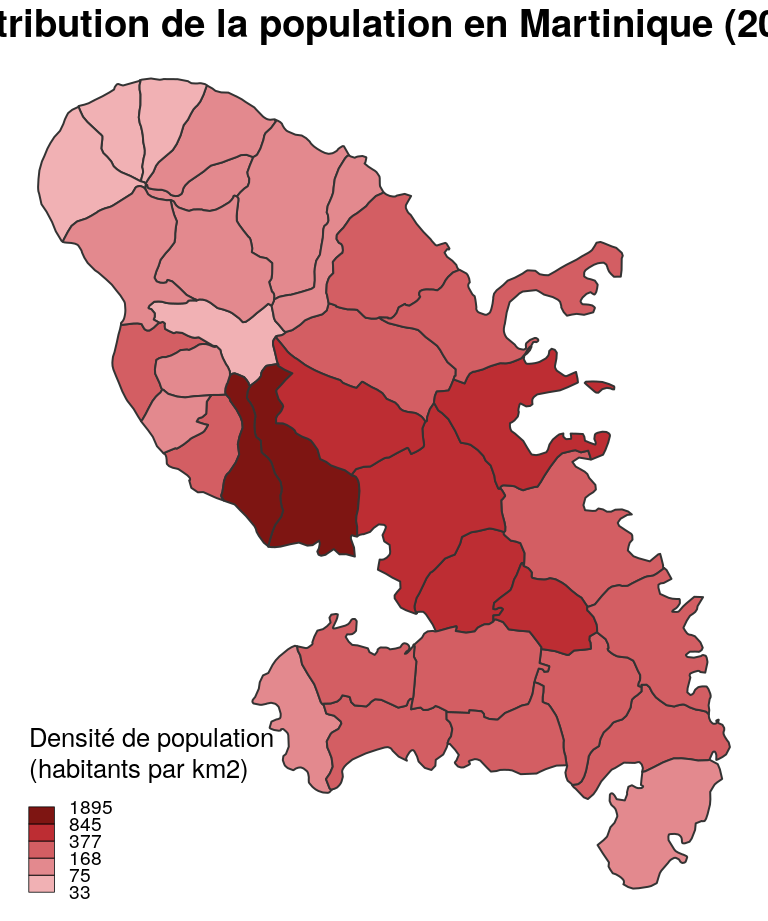
\includegraphics{Cartographie_avec_R_files/figure-latex/choro-1} \end{center}

\hypertarget{palettes-de-couleurs}{%
\section{Palettes de couleurs}\label{palettes-de-couleurs}}

\begin{Shaded}
\begin{Highlighting}[]
\KeywordTok{display.carto.all}\NormalTok{(}\DecValTok{20}\NormalTok{)}
\end{Highlighting}
\end{Shaded}

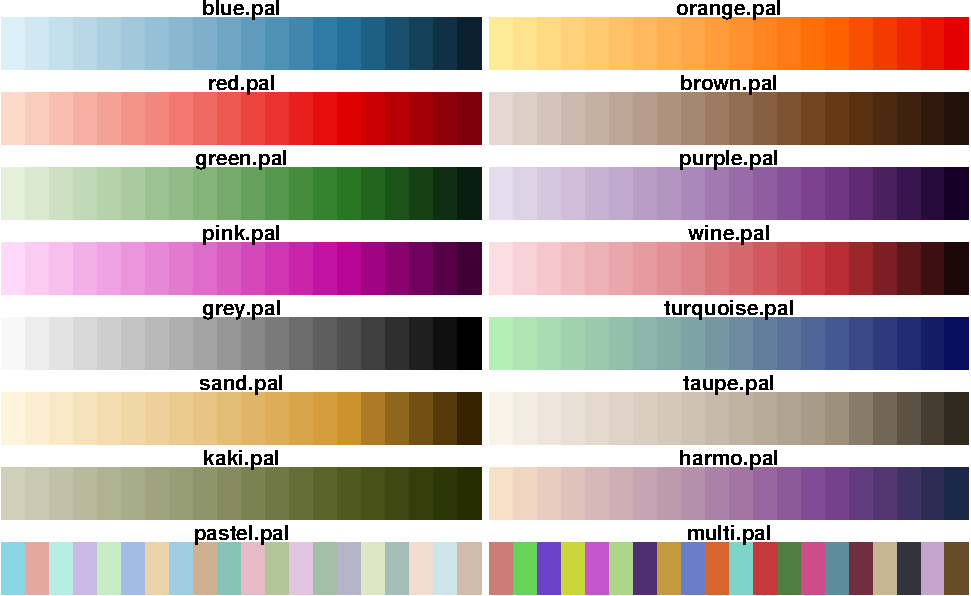
\includegraphics{Cartographie_avec_R_files/figure-latex/pal-1.pdf}

\begin{Shaded}
\begin{Highlighting}[]
\KeywordTok{display.carto.pal}\NormalTok{(}\StringTok{"orange.pal"}\NormalTok{)}
\end{Highlighting}
\end{Shaded}

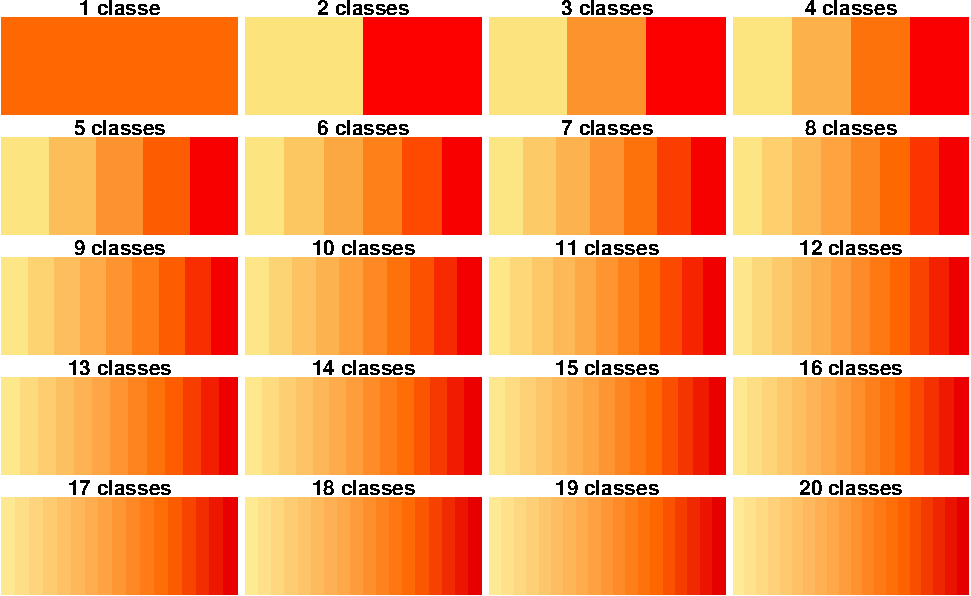
\includegraphics{Cartographie_avec_R_files/figure-latex/pal1-1.pdf}

\begin{Shaded}
\begin{Highlighting}[]
\NormalTok{mypal <-}\StringTok{ }\KeywordTok{carto.pal}\NormalTok{(}\DataTypeTok{pal1 =} \StringTok{"wine.pal"}\NormalTok{, }\DataTypeTok{n1 =} \DecValTok{7}\NormalTok{, }\DataTypeTok{pal2 =} \StringTok{"green.pal"}\NormalTok{, }\DataTypeTok{n2 =} \DecValTok{12}\NormalTok{,}
                   \DataTypeTok{middle =} \OtherTok{TRUE}\NormalTok{, }\DataTypeTok{transparency =} \OtherTok{TRUE}\NormalTok{)}
\NormalTok{k <-}\StringTok{ }\KeywordTok{length}\NormalTok{(mypal)}
\KeywordTok{image}\NormalTok{(}\DecValTok{1}\OperatorTok{:}\NormalTok{k, }\DecValTok{1}\NormalTok{, }\KeywordTok{as.matrix}\NormalTok{(}\DecValTok{1}\OperatorTok{:}\NormalTok{k), }\DataTypeTok{col=}\NormalTok{mypal, }\DataTypeTok{xlab =} \KeywordTok{paste}\NormalTok{(k,}\StringTok{" classes"}\NormalTok{,}\DataTypeTok{sep=}\StringTok{""}\NormalTok{),}
      \DataTypeTok{ylab =} \StringTok{""}\NormalTok{, }\DataTypeTok{xaxt =} \StringTok{"n"}\NormalTok{, }\DataTypeTok{yaxt =} \StringTok{"n"}\NormalTok{,}\DataTypeTok{bty =} \StringTok{"n"}\NormalTok{)}
\end{Highlighting}
\end{Shaded}

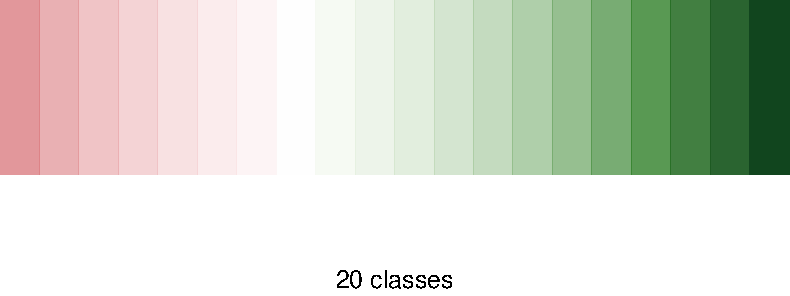
\includegraphics{Cartographie_avec_R_files/figure-latex/pal2-1.pdf}

\hypertarget{discretisations}{%
\section{Discrétisations}\label{discretisations}}

\begin{Shaded}
\begin{Highlighting}[]
\NormalTok{var <-}\StringTok{ }\NormalTok{mtq}\OperatorTok{$}\NormalTok{cagr}
\NormalTok{moy <-}\StringTok{ }\KeywordTok{mean}\NormalTok{(var)}
\NormalTok{med <-}\StringTok{ }\KeywordTok{median}\NormalTok{(var)}
\NormalTok{std <-}\StringTok{ }\KeywordTok{sd}\NormalTok{(var)}
\CommentTok{# Quantile intervals}
\NormalTok{breaks <-}\StringTok{ }\KeywordTok{getBreaks}\NormalTok{(}\DataTypeTok{v =}\NormalTok{ var, }\DataTypeTok{nclass =} \DecValTok{6}\NormalTok{, }\DataTypeTok{method =} \StringTok{"quantile"}\NormalTok{)}
\KeywordTok{hist}\NormalTok{(var, }\DataTypeTok{probability =} \OtherTok{TRUE}\NormalTok{, }\DataTypeTok{breaks =}\NormalTok{ breaks, }\DataTypeTok{main=}\StringTok{"quantiles"}\NormalTok{,}
     \DataTypeTok{col =} \KeywordTok{carto.pal}\NormalTok{(}\DataTypeTok{pal1 =} \StringTok{"wine.pal"}\NormalTok{,}\DecValTok{3}\NormalTok{, }\StringTok{"green.pal"}\NormalTok{, }\DecValTok{3}\NormalTok{))}
\KeywordTok{rug}\NormalTok{(var)}
\KeywordTok{abline}\NormalTok{(}\DataTypeTok{v =}\NormalTok{ med, }\DataTypeTok{col =} \StringTok{"blue"}\NormalTok{, }\DataTypeTok{lwd =} \DecValTok{3}\NormalTok{)}
\end{Highlighting}
\end{Shaded}

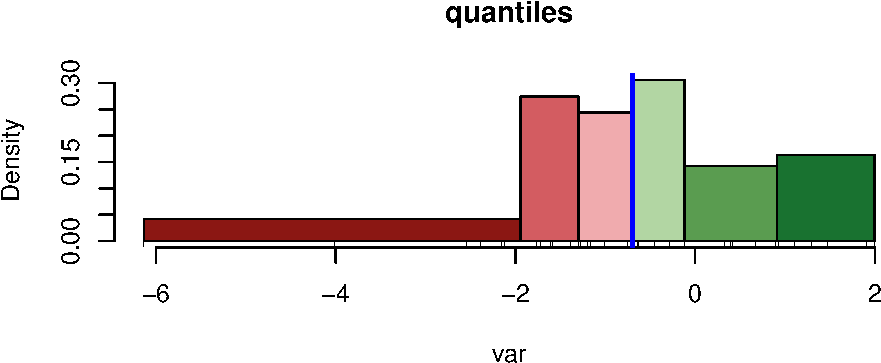
\includegraphics{Cartographie_avec_R_files/figure-latex/disc2-1.pdf}

\begin{Shaded}
\begin{Highlighting}[]
\CommentTok{# Mean and standard deviation (msd)}
\NormalTok{breaks <-}\StringTok{ }\KeywordTok{getBreaks}\NormalTok{(}\DataTypeTok{v =}\NormalTok{ var, }\DataTypeTok{method =} \StringTok{"msd"}\NormalTok{, }\DataTypeTok{k =} \DecValTok{1}\NormalTok{, }\DataTypeTok{middle =} \OtherTok{TRUE}\NormalTok{)}
\KeywordTok{hist}\NormalTok{(var, }\DataTypeTok{probability =} \OtherTok{TRUE}\NormalTok{, }\DataTypeTok{breaks =}\NormalTok{ breaks, }\DataTypeTok{main=}\StringTok{"moyenne / écart-type"}\NormalTok{,}
     \DataTypeTok{col =} \KeywordTok{carto.pal}\NormalTok{(}\DataTypeTok{pal1 =} \StringTok{"wine.pal"}\NormalTok{,}\DecValTok{3}\NormalTok{ , }\StringTok{"green.pal"}\NormalTok{, }\DecValTok{2}\NormalTok{, }\DataTypeTok{middle =} \OtherTok{TRUE}\NormalTok{))}
\KeywordTok{rug}\NormalTok{(var)}
\KeywordTok{abline}\NormalTok{(}\DataTypeTok{v =}\NormalTok{ moy, }\DataTypeTok{col =} \StringTok{"red"}\NormalTok{, }\DataTypeTok{lwd =} \DecValTok{3}\NormalTok{)}
\KeywordTok{abline}\NormalTok{(}\DataTypeTok{v =}\NormalTok{ moy }\OperatorTok{+}\StringTok{ }\FloatTok{0.5} \OperatorTok{*}\StringTok{ }\NormalTok{std, }\DataTypeTok{col =} \StringTok{"blue"}\NormalTok{, }\DataTypeTok{lwd =} \DecValTok{3}\NormalTok{)}
\KeywordTok{abline}\NormalTok{(}\DataTypeTok{v =}\NormalTok{ moy }\OperatorTok{-}\StringTok{ }\FloatTok{0.5} \OperatorTok{*}\StringTok{ }\NormalTok{std, }\DataTypeTok{col =} \StringTok{"blue"}\NormalTok{, }\DataTypeTok{lwd =} \DecValTok{3}\NormalTok{)}
\end{Highlighting}
\end{Shaded}

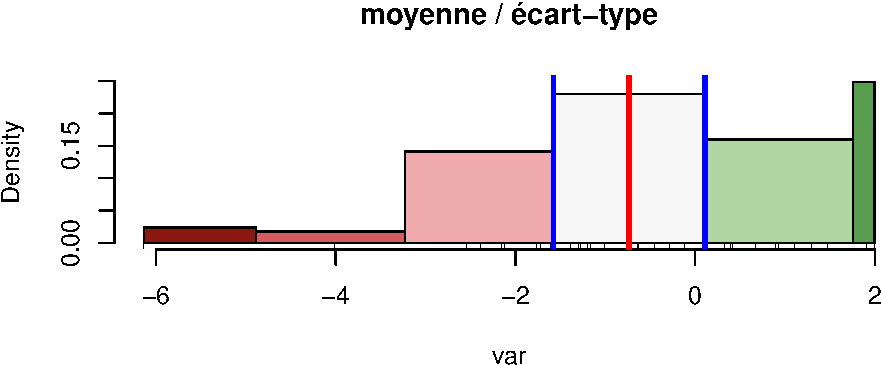
\includegraphics{Cartographie_avec_R_files/figure-latex/disc3-1.pdf}

\hypertarget{combinaisons}{%
\section{Combinaisons}\label{combinaisons}}

\begin{Shaded}
\begin{Highlighting}[]
\KeywordTok{plot}\NormalTok{(}\KeywordTok{st_geometry}\NormalTok{(mtq), }\DataTypeTok{col =} \StringTok{"lightblue4"}\NormalTok{,}
     \DataTypeTok{border =} \StringTok{"lightblue3"}\NormalTok{, }\DataTypeTok{bg =} \StringTok{"lightblue1"}\NormalTok{)}
\KeywordTok{propSymbolsChoroLayer}\NormalTok{(}\DataTypeTok{x =}\NormalTok{ mtq, }\DataTypeTok{var=} \StringTok{"P13_POP"}\NormalTok{,}
                 \DataTypeTok{legend.var.title.txt =} \StringTok{"Total}\CharTok{\textbackslash{}n}\StringTok{population (2013)"}\NormalTok{,}
           \DataTypeTok{var2 =} \StringTok{"cagr"}\NormalTok{, }\DataTypeTok{legend.var.pos =} \StringTok{"bottomleft"}\NormalTok{,}
           \DataTypeTok{breaks =} \KeywordTok{c}\NormalTok{(}\OperatorTok{-}\FloatTok{6.14}\NormalTok{,}\OperatorTok{-}\DecValTok{2}\NormalTok{,}\OperatorTok{-}\DecValTok{1}\NormalTok{,}\DecValTok{0}\NormalTok{,}\DecValTok{1}\NormalTok{,}\DecValTok{2}\NormalTok{),}
           \DataTypeTok{col =} \KeywordTok{c}\NormalTok{(}\StringTok{"#135D89"}\NormalTok{, }\StringTok{"#4D95BA"}\NormalTok{, }\StringTok{"#96D1EA"}\NormalTok{, }\StringTok{"#FCDACA"}\NormalTok{, }\StringTok{"#EC4E49"}\NormalTok{),}
           \DataTypeTok{legend.var2.title.txt =} \StringTok{"Compound annual}\CharTok{\textbackslash{}n}\StringTok{growth rate"}\NormalTok{)}
\CommentTok{# Title}
\KeywordTok{title}\NormalTok{(}\DataTypeTok{main =} \StringTok{"Evolution de la population"}\NormalTok{)}
\end{Highlighting}
\end{Shaded}

\begin{center}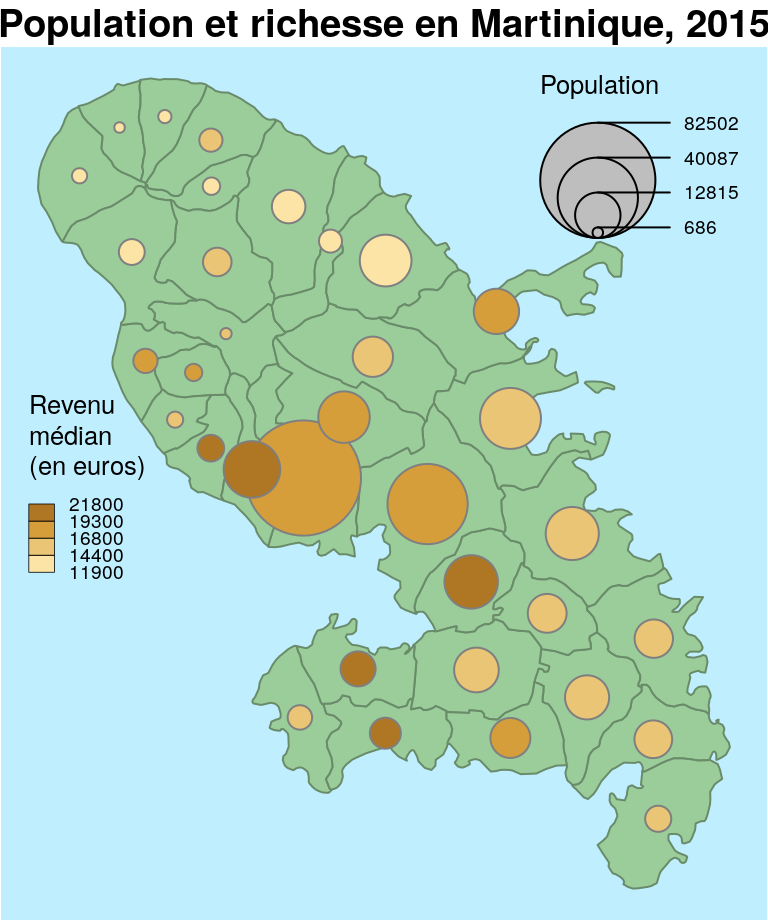
\includegraphics{Cartographie_avec_R_files/figure-latex/choroprop-1} \end{center}

\hypertarget{labels}{%
\section{Labels}\label{labels}}

\begin{Shaded}
\begin{Highlighting}[]
\KeywordTok{plot}\NormalTok{(}\KeywordTok{st_geometry}\NormalTok{(mtq), }\DataTypeTok{col =} \StringTok{"darkseagreen3"}\NormalTok{, }\DataTypeTok{border =} \StringTok{"darkseagreen4"}\NormalTok{,}
     \DataTypeTok{bg =} \StringTok{"#A6CAE0"}\NormalTok{)}
\KeywordTok{labelLayer}\NormalTok{(}\DataTypeTok{x =}\NormalTok{ mtq, }\DataTypeTok{txt =} \StringTok{"LIBGEO"}\NormalTok{, }\DataTypeTok{col=} \StringTok{"black"}\NormalTok{, }\DataTypeTok{cex =} \FloatTok{0.7}\NormalTok{, }\DataTypeTok{font =} \DecValTok{4}\NormalTok{,}
           \DataTypeTok{halo =} \OtherTok{TRUE}\NormalTok{, }\DataTypeTok{bg =} \StringTok{"white"}\NormalTok{, }\DataTypeTok{r =} \FloatTok{0.1}\NormalTok{, }\DataTypeTok{overlap =} \OtherTok{FALSE}\NormalTok{, }
           \DataTypeTok{show.lines =} \OtherTok{FALSE}\NormalTok{)}
\end{Highlighting}
\end{Shaded}

\begin{center}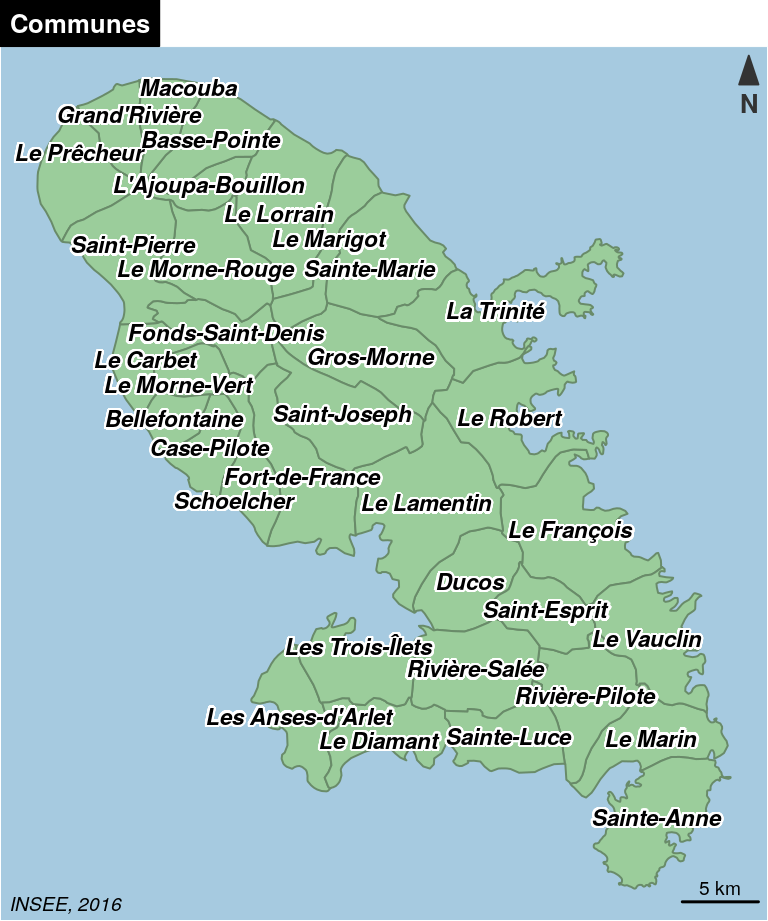
\includegraphics{Cartographie_avec_R_files/figure-latex/labs-1} \end{center}

\hypertarget{les-donnees-osm}{%
\section{Les données OSM}\label{les-donnees-osm}}

\hypertarget{donnees-vectorielles}{%
\subsection{Données vectorielles}\label{donnees-vectorielles}}

\hypertarget{donnees-raster}{%
\subsection{Données raster}\label{donnees-raster}}

\begin{Shaded}
\begin{Highlighting}[]
\NormalTok{tiles <-}\StringTok{ }\KeywordTok{getTiles}\NormalTok{(}\DataTypeTok{x =}\NormalTok{ mtq, }\DataTypeTok{type =} \StringTok{"osm"}\NormalTok{, }\DataTypeTok{crop=}\NormalTok{T, }\DataTypeTok{zoom =} \DecValTok{11}\NormalTok{)}
\KeywordTok{tilesLayer}\NormalTok{(tiles)}
\KeywordTok{plot}\NormalTok{(}\KeywordTok{st_geometry}\NormalTok{(mtq), }\DataTypeTok{add=}\NormalTok{T)}
\end{Highlighting}
\end{Shaded}

\begin{center}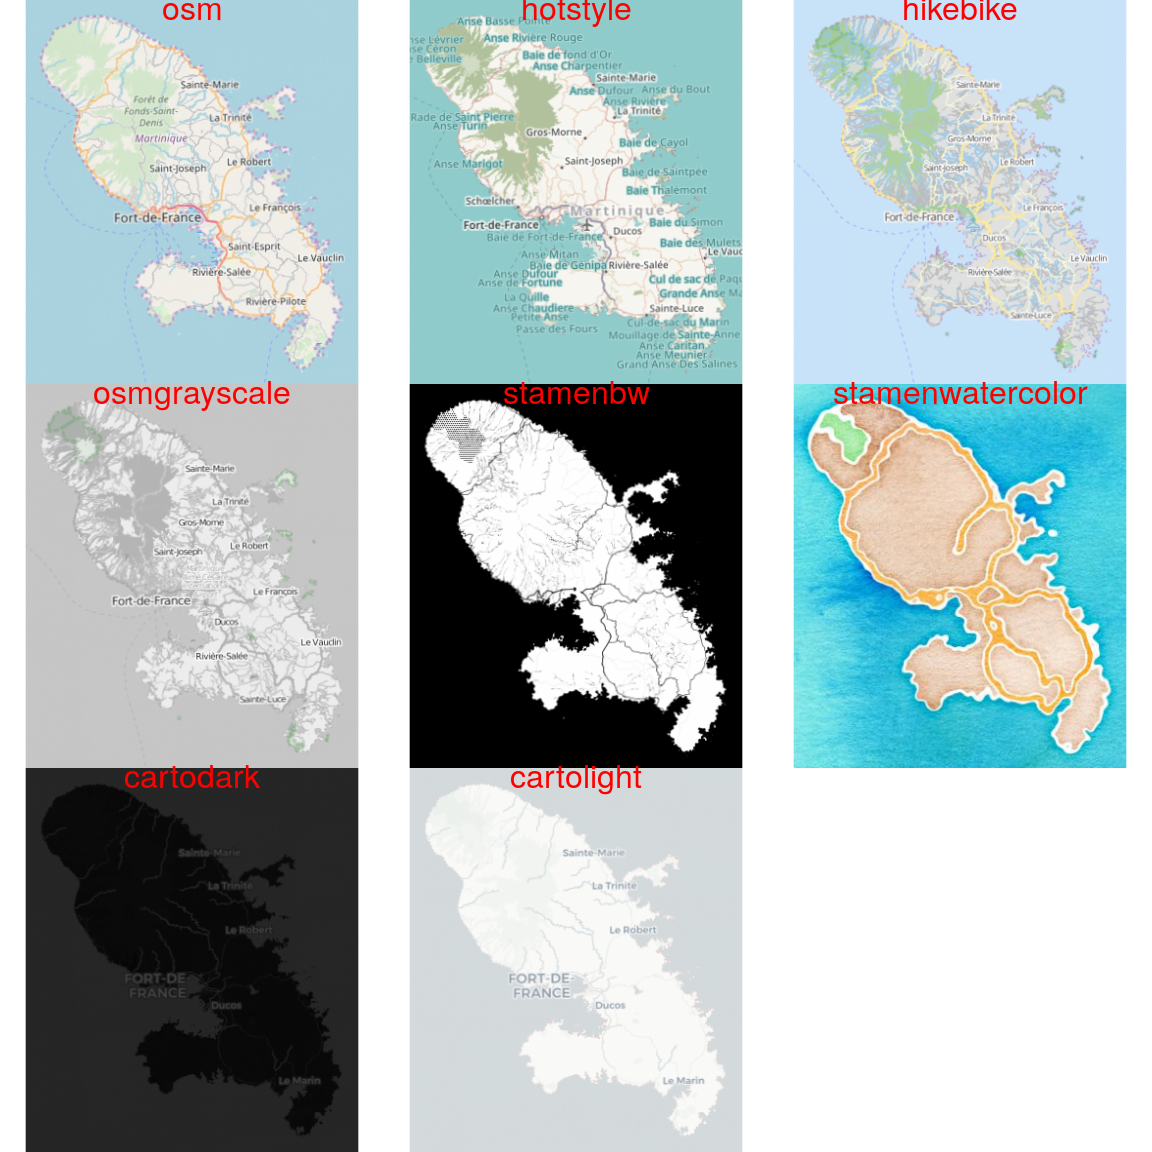
\includegraphics{Cartographie_avec_R_files/figure-latex/osm-1} \end{center}

\hypertarget{cartographie-interactive}{%
\section{Cartographie interactive}\label{cartographie-interactive}}

leaflet / mapview

\hypertarget{geocodage-dadresses}{%
\section{Géocodage d'adresses}\label{geocodage-dadresses}}

\hypertarget{creation-de-cartons}{%
\section{Création de cartons}\label{creation-de-cartons}}

\hypertarget{jour3}{%
\chapter{Cartographie thématique avancée}\label{jour3}}

\hypertarget{les-anamorphoses}{%
\section{Les anamorphoses}\label{les-anamorphoses}}

Voir : \href{https://neocarto.hypotheses.org/366}{Les anamorphoses cartographiques}\\
\emph{Nicolas Lambert, 2015}

``L'anamorphose classique est une représentation des États (ou de mailles quelconques) par \textbf{des rectangles ou des polygones quelconques} en fonction d'une \textbf{quantité} qui leur est rattaché.''

``On s'efforce de \textbf{garder l'arrangement général} des mailles ou la silhouette du continent.''

\emph{Brunet, R., Ferras, R., \& Théry, H. (1993). Les mots de la géographie: dictionnaire critique (No.~03) 911 BRU).}

\hypertarget{les-cartogrammes-de-dorling}{%
\subsection{Les cartogrammes de Dorling}\label{les-cartogrammes-de-dorling}}

La taille des cercles est proportionnelle à une variable.

La position des cercles est définie selon les positions de départ.

\emph{Dorling, Daniel (1996): Area Cartograms: Their Use and Creation, Concepts and Techniques in Modern Geography (CATMOG), 59}

\hypertarget{le-principe}{%
\subsection{Le principe}\label{le-principe}}

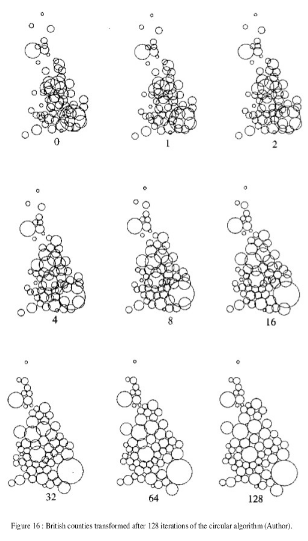
\includegraphics{img/dorling1.png}

\hypertarget{exemple}{%
\subsection{Exemple}\label{exemple}}

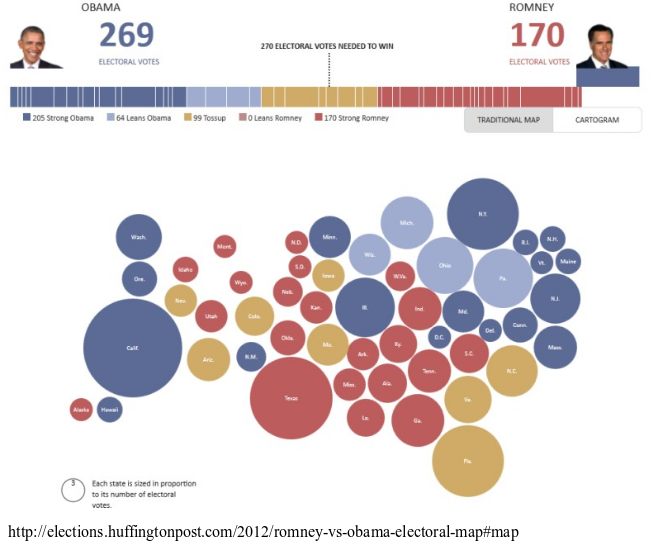
\includegraphics{img/dorling2.png}
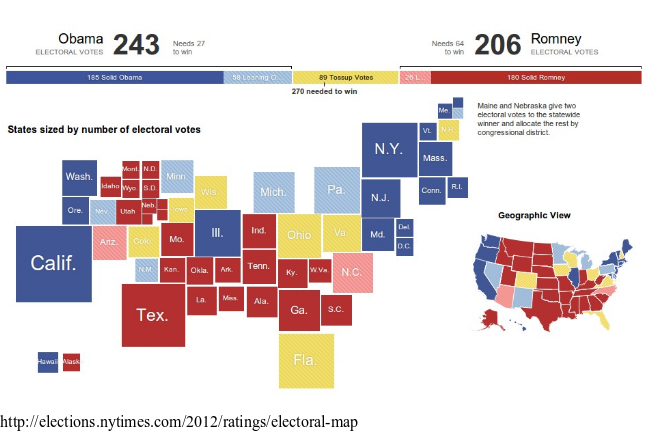
\includegraphics{img/dorling3.png}

\hypertarget{precautions-demploi}{%
\subsection{Précautions d'emploi}\label{precautions-demploi}}

- On identifie assez mal l'espace\\
On peut nommer les cercles pour se repérer\\
On peut s'aider de la couleur pour faire des clusters et mieux identifier les blocks géographiques

+ La perception de la quantité est très bonne.\\
Les tailles de cercles sont vraiment comparables

\hypertarget{les-cartogrammes-non-continus}{%
\subsection{Les cartogrammes non continus}\label{les-cartogrammes-non-continus}}

La taille des polygones est proportionnelle à une variable.

L'agencement des polygones les uns par rapport aux autres est conservée.

La forme des polygones est ressemblante.

\hypertarget{exemple-1}{%
\subsection{Exemple}\label{exemple-1}}

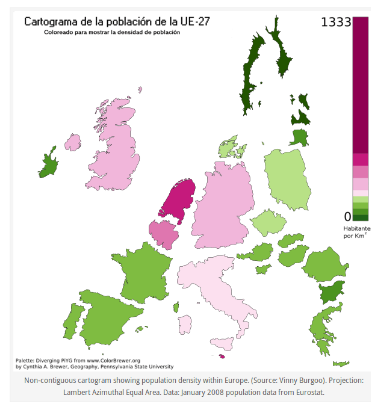
\includegraphics{img/nc.png}

\hypertarget{precautions-demploi-1}{%
\subsection{Précautions d'emploi}\label{precautions-demploi-1}}

- Non contigu, la topologie est perdue.

+ La conservation de la forme des polygones est optimisée.

\hypertarget{les-cartogrammes-continus}{%
\subsection{Les cartogrammes continus}\label{les-cartogrammes-continus}}

La taille des polygones est proportionnelle à une variable.

L'agencement des polygones les uns par rapport aux autres est conservée.

Pour conserver la contiguité, la forme des polygones est fortement transformée.

\hypertarget{exemple-2}{%
\subsection{Exemple}\label{exemple-2}}

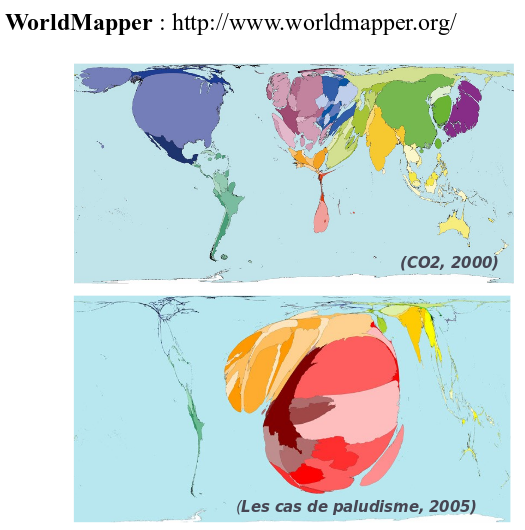
\includegraphics{img/c.png}

\hypertarget{precautions-demploi-2}{%
\subsection{Précautions d'emploi}\label{precautions-demploi-2}}

- Par rapport aux anamorphoses non contigues, la forme des polygones est fortement distordue.

+ C'est une ``vraie carte de géographie'' : la topologie et la contiguité sont conservées.

\hypertarget{interets-des-anamorphoses}{%
\subsection{Interêts des anamorphoses}\label{interets-des-anamorphoses}}

Représentation cartographique perçue comme \textbf{innovante} (même si la methode date de 40 ans)

Image très généralisée qui rend bien compte des \textbf{quantités} et des \textbf{gradiants}.

Une vraie image de \textbf{communication} : \textbf{provoque}, suscite \textbf{l'intérêt}, véhicule un \textbf{message} fort, \textbf{interpelle}.

\hypertarget{faiblesses-des-anamorphoses}{%
\subsection{Faiblesses des anamorphoses}\label{faiblesses-des-anamorphoses}}

Perte des \textbf{repères visuels} (difficile de retrouver son pays, ou sa région sur la carte).

Ne permet pas de connaître les \textbf{situations locales}.

Demande un \textbf{effort de lecture}.

\textbf{Gestion des données manquantes}

\hypertarget{les-grilles-regulieres}{%
\section{Les grilles régulières}\label{les-grilles-regulieres}}

Par une série d'opération SIG assez simple il est possible de transformer des données d'un maillage initial vers un maillage régulier plus neutre et plus simple.

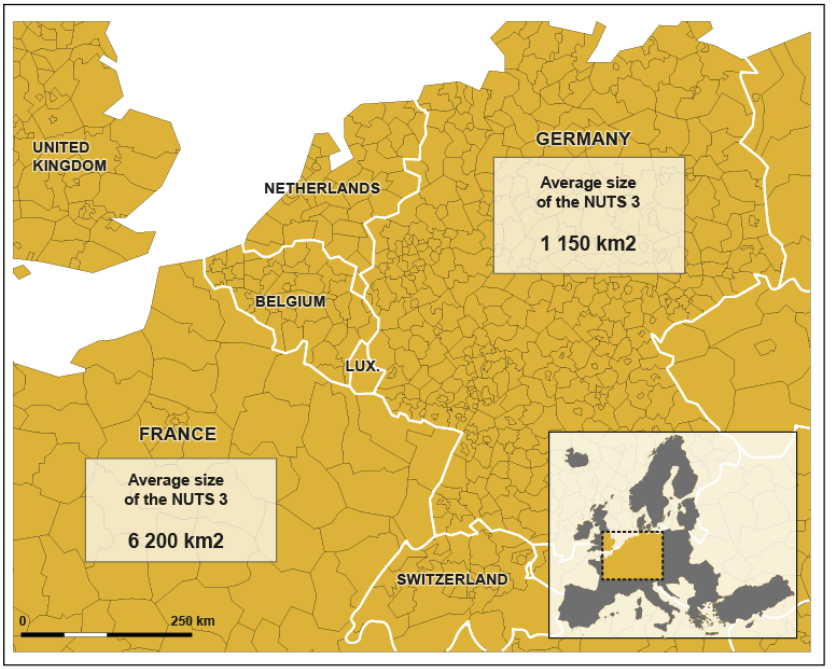
\includegraphics{img/maup.png}

\hypertarget{exemples}{%
\subsection{Exemples}\label{exemples}}

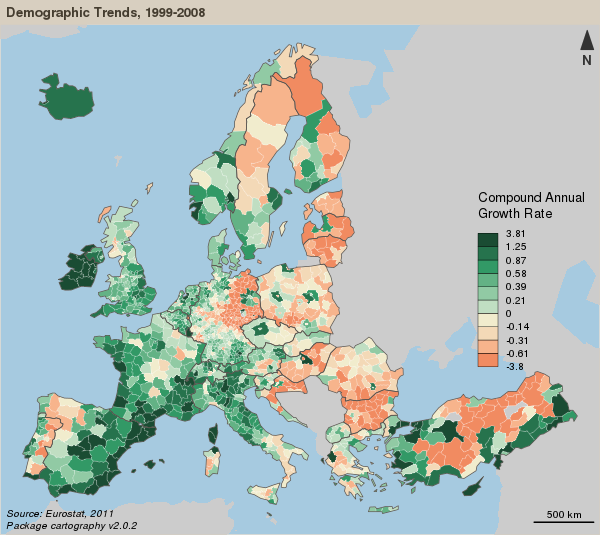
\includegraphics{img/pregrid.png}

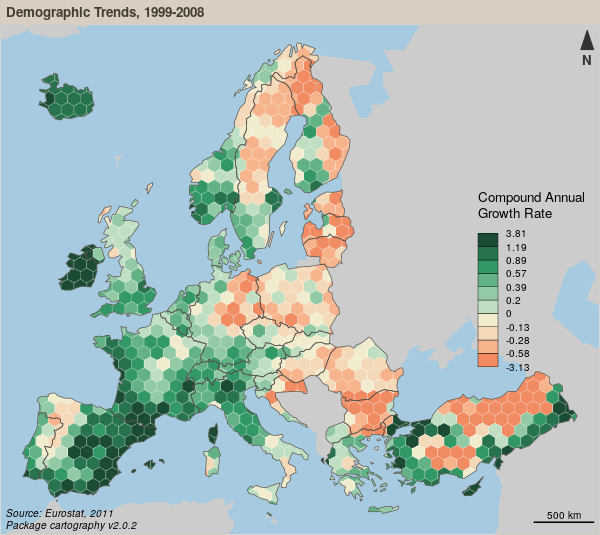
\includegraphics{img/grid.png}

\hypertarget{precautions-demploi-3}{%
\subsection{Précautions d'emploi}\label{precautions-demploi-3}}

- Perte de précision, maillage sans signification.\\
La version simple (au prorata de la surface), implique une equirépartition du phénomène dans chaque unités.

+ Permet la comparaison de maillages différents, à plusieurs dates ou de différentes sources.

\hypertarget{les-discontinuites}{%
\section{Les discontinuités}\label{les-discontinuites}}

Ce type de représentation permet de souligner cartographiquement les discontinuités territoriales d'un phénomène.

L'accent est porter sur ce qui distingue des territoires.

Pour chaque frontière nous calculons le rapports ou la différence des valeurs des polygones de part et d'autre. Puis nous représentons la frontière par un figuré d'autant plus épais que la différence est forte.

Il est souvent bénéfique de coupler ce type de représentation à une représentation choroplèthe (pour comprendre le sens des discontinuités).
\#\#\# Exemples

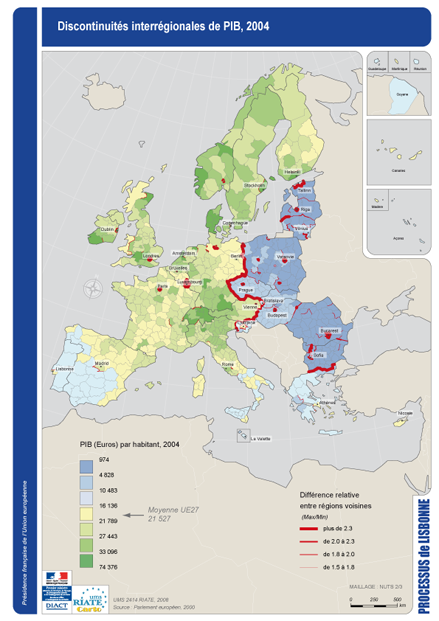
\includegraphics{img/disc1.png}

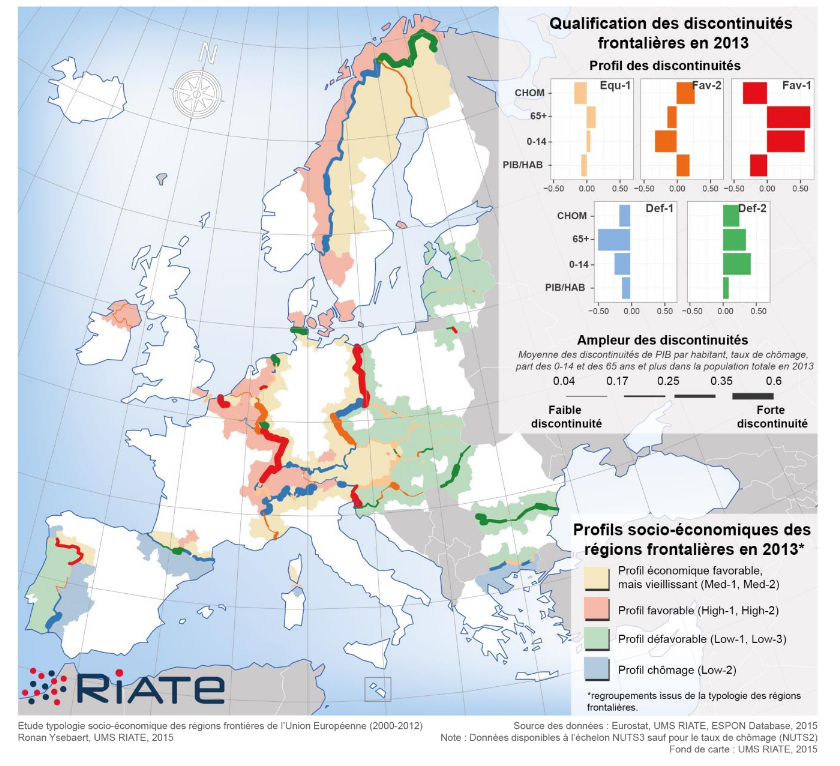
\includegraphics{img/disc2.png}

\hypertarget{precautions-demploi-4}{%
\subsection{Précautions d'emploi}\label{precautions-demploi-4}}

- Ces cartes ne sont pas évidentes à paramétrer.\\
Le choix des critères (seuil, type de différences\ldots{}) va fortement influencer la représentation.\\
En fonction du maillage la lisibilité peut être faible.

+ Représentation très puissante pour montrer les inégalités.

\hypertarget{les-lissages}{%
\section{Les lissages}\label{les-lissages}}

L'idée principale du lissage est de filtrer l'information pour révéler des structures spatiales sous-jacentes.

C'est un ensemble de méthodes qui consistent à affecter aux points que l'on observe une valeur prenant en compte les valeurs de leur voisinnage.

Il existe plusieurs méthodes de lissage (kde, potentiels\ldots{}) plus ou moins paramétrables.

Cette méthode permet de passer représentations ponctuelles à une représentation continu

\hypertarget{exemples-1}{%
\subsection{Exemples}\label{exemples-1}}

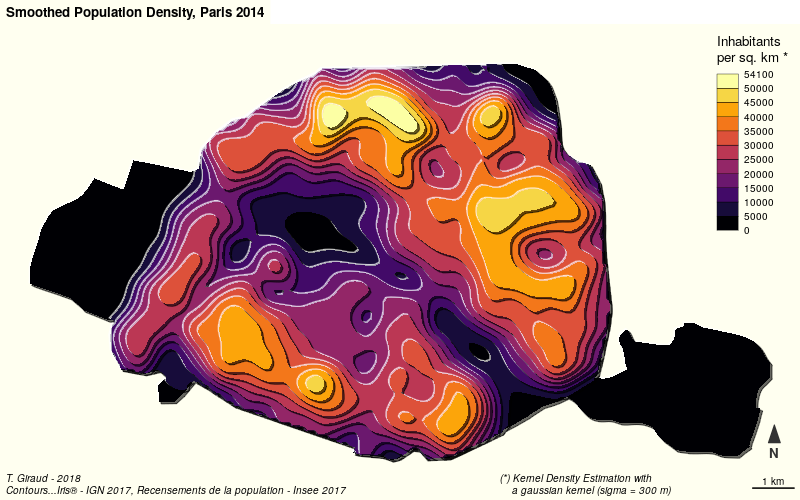
\includegraphics{img/liss1.png}
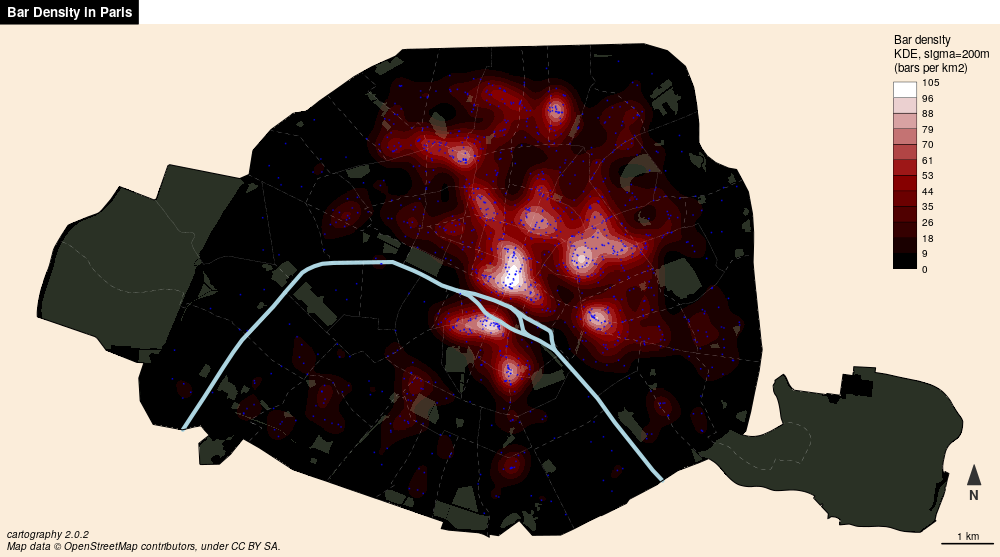
\includegraphics{img/liss2.png}

\hypertarget{precautions-demploi-5}{%
\subsection{Précautions d'emploi}\label{precautions-demploi-5}}

- Il est difficile de paramétrer correctement les fonctions de lissages.\\
Elles doivent s'appuyer sur des hypothèses de comportement dans l'espace.\\
La compréhension par un public large n'est pas évidente, il faut alors simplifier les légendes, la présentation de la méthode.

+ Permet de faire ressortir des phénomènes spatiaux sous-jacents invisibles directement.\\
Les cartes produites attirent l'oeil par leur originalité.\\
Cette méthode permet de passer d'une représentation ponctuelle ou discontuinue (dans un maillage) à une représentation continue s'affranchissant des maillages existants.

\hypertarget{kde}{%
\subsection{KDE}\label{kde}}

\hypertarget{stewart}{%
\subsection{Stewart}\label{stewart}}

\href{https://cran.r-project.org/web/packages/SpatialPosition/vignettes/StewartExample.html}{Vignette du package SpatialPosition}

\hypertarget{d}{%
\section{3D}\label{d}}

\hypertarget{linemap}{%
\subsection{linemap}\label{linemap}}

\begin{Shaded}
\begin{Highlighting}[]
\KeywordTok{library}\NormalTok{(linemap)}
\KeywordTok{library}\NormalTok{(sf)}
\KeywordTok{data}\NormalTok{(}\StringTok{"popOcc"}\NormalTok{)}
\KeywordTok{data}\NormalTok{(}\StringTok{"occitanie"}\NormalTok{)}
\NormalTok{opar <-}\StringTok{ }\KeywordTok{par}\NormalTok{(}\DataTypeTok{mar=}\KeywordTok{c}\NormalTok{(}\DecValTok{0}\NormalTok{,}\DecValTok{0}\NormalTok{,}\DecValTok{0}\NormalTok{,}\DecValTok{0}\NormalTok{), }\DataTypeTok{bg =} \StringTok{"ivory2"}\NormalTok{)}
\NormalTok{bb <-}\StringTok{ }\KeywordTok{st_bbox}\NormalTok{(occitanie)}
\KeywordTok{plot}\NormalTok{(}\KeywordTok{st_geometry}\NormalTok{(occitanie), }\DataTypeTok{col=}\StringTok{"ivory1"}\NormalTok{, }\DataTypeTok{border =} \OtherTok{NA}\NormalTok{)}
\KeywordTok{linemap}\NormalTok{(}\DataTypeTok{x =}\NormalTok{ popOcc, }\DataTypeTok{var =} \StringTok{"pop"}\NormalTok{, }\DataTypeTok{k =} \FloatTok{2.5}\NormalTok{, }\DataTypeTok{threshold =} \DecValTok{50}\NormalTok{,}
        \DataTypeTok{col =} \StringTok{"ivory1"}\NormalTok{, }\DataTypeTok{border =} \StringTok{"ivory4"}\NormalTok{, }\DataTypeTok{lwd =} \FloatTok{0.6}\NormalTok{, }\DataTypeTok{add =} \OtherTok{TRUE}\NormalTok{)}
\KeywordTok{text}\NormalTok{(}\DataTypeTok{x =}\NormalTok{ bb[}\DecValTok{1}\NormalTok{], }\DataTypeTok{y =}\NormalTok{ bb[}\DecValTok{4}\NormalTok{],}\DataTypeTok{adj =} \KeywordTok{c}\NormalTok{(}\DecValTok{0}\NormalTok{,}\DecValTok{1}\NormalTok{),}
     \DataTypeTok{labels =} \StringTok{"Répartition de la}\CharTok{\textbackslash{}n}\StringTok{population}\CharTok{\textbackslash{}n}\StringTok{en Occitanie"}\NormalTok{,  }
     \DataTypeTok{col =} \StringTok{"ivory4"}\NormalTok{, }\DataTypeTok{font =} \DecValTok{2}\NormalTok{,  }\DataTypeTok{cex =} \FloatTok{1.8}\NormalTok{)}
\CommentTok{# add sources}
\NormalTok{mapsources <-}\StringTok{"Timothée Giraud}\CharTok{\textbackslash{}n}\StringTok{R 3.4.1, cartography 2.0.0, linemap 0.1.0}\CharTok{\textbackslash{}n}\StringTok{Données carroyées à 1 kilomètre, INSEE 2010"}
\KeywordTok{text}\NormalTok{(}\DataTypeTok{x =}\NormalTok{ bb[}\DecValTok{3}\NormalTok{], }\DataTypeTok{y =}\NormalTok{ bb[}\DecValTok{2}\NormalTok{],}\DataTypeTok{labels =}\NormalTok{ mapsources,  }
     \DataTypeTok{col =} \StringTok{"ivory4"}\NormalTok{, }\DataTypeTok{font =} \DecValTok{3}\NormalTok{, }\DataTypeTok{adj =} \KeywordTok{c}\NormalTok{(}\DecValTok{1}\NormalTok{,}\DecValTok{0}\NormalTok{), }\DataTypeTok{cex =} \FloatTok{0.6}\NormalTok{ )}
\end{Highlighting}
\end{Shaded}

\begin{center}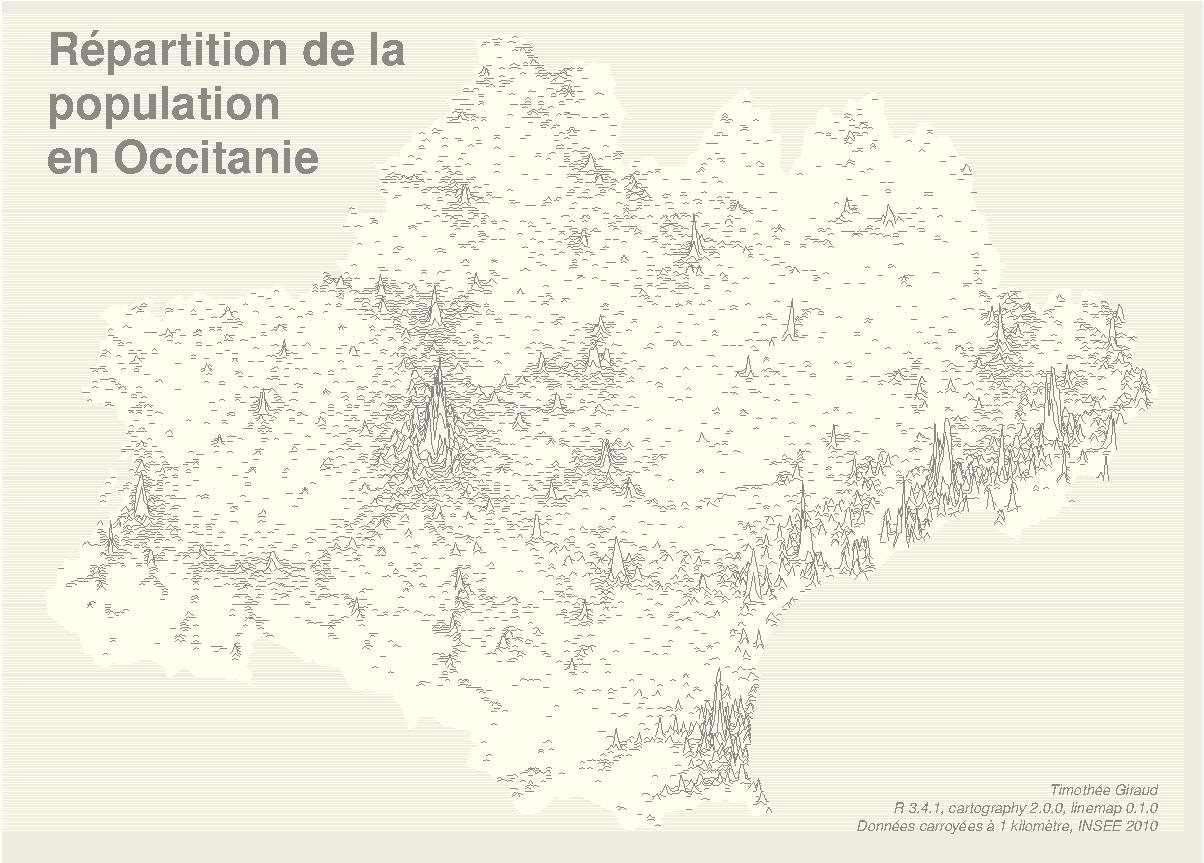
\includegraphics{Cartographie_avec_R_files/figure-latex/lines-1} \end{center}

\hypertarget{rayshader}{%
\subsection{rayshader}\label{rayshader}}

\bibliography{book.bib,packages.bib}


\end{document}
